\documentclass{article}
\usepackage[T1]{fontenc}
\usepackage[utf8]{inputenc}
\usepackage[margin=1in]{geometry}
\usepackage{fancyhdr} 
\usepackage{listings}
\usepackage{algorithm}
\usepackage[noend]{algorithmic}
\usepackage{amsmath, amsthm, amssymb, amsfonts}
\usepackage{graphicx}
\usepackage[dvipsnames]{xcolor}
\usepackage{xy}
\usepackage{url}
\usepackage{parskip}
\usepackage{comment}
\usepackage{setspace}
\usepackage{enumerate}
\usepackage{multirow}
\usepackage{hyperref}
\usepackage{caption}
\usepackage{subcaption}
\usepackage{booktabs}
\usepackage{wrapfig}
\usepackage{times}

\captionsetup[figure]{font={small,it}}

\usepackage[backend=biber,style=numeric,sortcites,maxbibnames=99]{biblatex}
\addbibresource{references.bib}

\newcommand{\HRule}{\rule{\linewidth}{0.5mm}}
\newcommand{\Hrule}{\rule{\linewidth}{0.3mm}}
\newcommand{\classnum}{CS-GY 6313 B}

\makeatletter% since there's an at-sign (@) in the command name
\renewcommand{\@maketitle}{%
  \parindent=0pt% don't indent paragraphs in the title block
  \centering
  {\Large \bfseries\textsc{\@title}}
  \HRule\par%
  \textit{\@author \hfill \classnum}
  \par
}
\makeatother% resets the meaning of the at-sign (@)

\title{Assignment 4: Data Viz for Advocacy}
\author{Sanyukta Tuti}
% \classnum

\begin{document}
  \maketitle % prints the title block
  \thispagestyle{empty}
  % \vspace{-15pt}

\section{Introduction}
\label{sec:sec1}

\maketitle

Plastic pollution is a pressing environmental challenge, with production skyrocketing from 2 million tonnes in 1950 to over 450 million tonnes today. Despite its versatility across industries, improper management results in 1–2 million tonnes of plastic entering oceans annually, devastating wildlife and ecosystems. These visualizations explore the crisis through economic growth, waste management, regional disparities, and plastic types, emphasizing the urgency for action utilizing the OECD (2022), Global Plastics Outlook dataset \cite{dataset}. The goal is to answer the following questions:

\begin{enumerate}
    \item \textit{"What are the major years of change in plastic production, and how do they correlate with industrial or environmental trends?"}
    \item \textit{"What is the global disparity in plastic waste generation and plastic waste management?"}
    \item \textit{"What can be done to reduce the specific plastic waste types identified in regions?"}
\end{enumerate}

\begin{figure}[ht] 
    \centering
    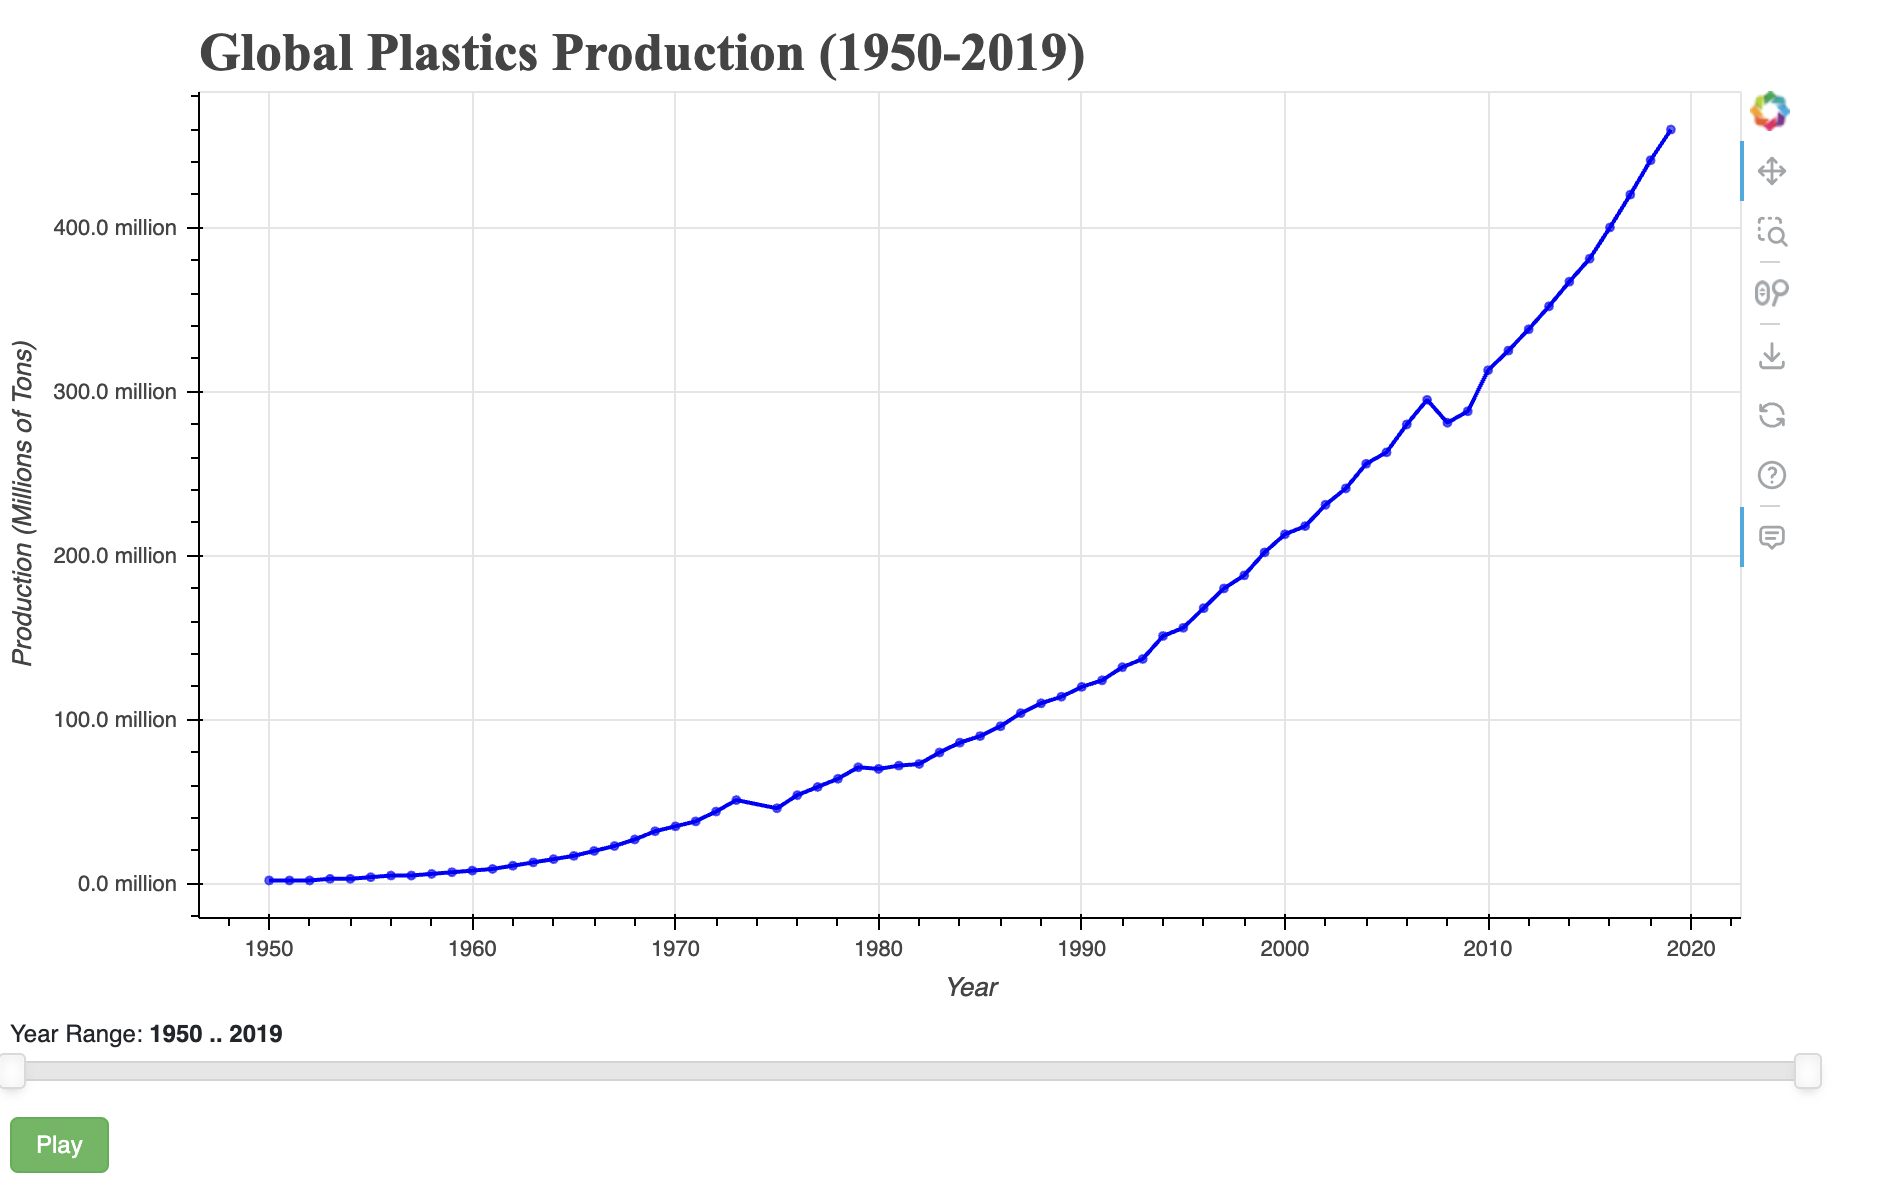
\includegraphics[width=0.75\textwidth]{st5442_assignment4/fig/Layout1.png}
    \caption{
        From Progress to Pollution-What are the major years of change in plastic production?
    }
    \label{fig:Import}
\end{figure}


\section{Visualization on Progress to Pollution: Global Plastics Production (1950-2019)}

\subsection{Design Rationale}

\subsubsection{Data Preprocessing}
The dataset records annual plastic production (1950–2019) in raw tons. Preprocessing scales these values to millions of tons for clearer interpretation and effective visualization.

\subsubsection{Choice of Visualization}
\begin{itemize}
    \item A line plot is chosen to show the trend of plastic production over time making it suitable for depicting trends over a long period (1950-2019).
\end{itemize}

\subsubsection{Interaction Techniques}
\begin{itemize}
    \item \textbf{Range Slider:} Users can slide the range slider to select a specific time range (from 1950 to 2019). This will update the plot to show only the data within the selected range.
    \item \textbf{Play Button:} Clicking the play button initiates the animation, which moves the range slider automatically through the years from 1950 to 2019.
    \item \textbf{Hover Tool:} By hovering over any point on the line graph or the circles, users can see the exact year and the corresponding plastic production value.
\end{itemize}

\section{Visualization on Tracing the Footprints of Plastic: Industrial Growth and Sustainability (1990-2019)}

\subsection{Design Rationale}

\subsubsection{Data Preprocessing}
\begin{itemize}
    \item To make the data more manageable and meaningful, I scaled the production values to millions of tonnes (using \texttt{.div(1\_000\_000)}), ensuring that the visualization’s axes are easier to interpret.
    \item I used cumulative summation (\texttt{cumsum(axis=1)}) to stack the production values, allowing us to see the relative contribution of each sector within each year. 
\end{itemize}

\subsubsection{Choice of Visualization}
\textbf{Stacked Area Plot:} A stacked area plot allows us to track the changes in production over time for each sector and observe how the sector’s share of total plastic production has evolved. 

\subsubsection{Interaction Techniques}
\begin{itemize}
\item\textbf{Dropdown Menu for Highlighting Sectors:} The user can select a sector from the dropdown menu to toggle the visibility on a specific sector (such as Packaging or Transportation) and see how its production compares to the others. 
\item \textbf{RangeSlider for Year Filtering:} The user can adjust the range slider to select a range of years (from 1990 to 2019). This filters the data to show plastic production only for the selected years.
\item \textbf{Play Button for Animation:} Clicking the "Play" button animates the plot by incrementally advancing the year range. The animation progresses from 1990 to 2019.
\end{itemize}

\section{Visualization on Plastic Borders: A Crisis Without Boundaries (Plastic Waste Generation, 2019)}

\subsection{Design Rationale}

\subsubsection{Data Preprocessing}
\textbf{Filtering Data by Year:} The dataset includes multiple years, but we focus on 2019 to create a snapshot of plastic waste generation in that year to ensures that the visualization focuses on the specific distribution for 2019, which is the intended point of analysis.

\subsubsection{Choice of Visualization}
\textbf{Choropleth Map:} A geographical map is chosen to show plastic waste generation, with each country represented as a polygon filled with color corresponding to its plastic waste generation.

\subsubsection{Interaction Techniques}
\textbf{Interactive Legend:}
\begin{itemize}
    \item \textbf{How to Use:} Users can select one or more bins in the legend to filter the countries shown on the map, allowing users to focus on countries with specific levels of plastic waste generation.
    \item \textbf{Hover Tool:} When the user hovers their mouse over a country, a tooltip will display the country’s name and its plastic waste generation value.
\end{itemize}

\section{Visualization on Linking Prosperity and Pollution: A Paradox in Plastic Management}

\subsection{Design Rationale}

\subsubsection{Data Preprocessing}
\begin{itemize}
        \item \textbf{Data Cleaning:} Columns were renamed for clarity, and only relevant columns were retained from the datasets. Missing or invalid GDP values were converted to numeric or handled appropriately to avoid errors.
        \item \textbf{Data Merging:} The datasets were merged using the country name to establish a relationship between GDP per capita\cite{GDP} and mismanaged plastic waste per capita. An outer join ensured that all countries with valid data were included.
        \item \textbf{Continent Mapping:} Countries were categorized by continent using a custom mapping function. A unique color was assigned to each continent for quick visual grouping. The choice of distinct and intuitive colors ensured clarity.
\end{itemize}

\subsubsection{Choice of Visualization}
A \textbf{scatter plot} was chosen to compare two continuous variables (GDP and mismanaged waste) and highlight correlations, and outliers to provide an intuitive representation of the relationship between wealth and waste management.

\subsubsection{Interaction Techniques}
\textbf{Hover Tool:} Hover over any data point to reveal detailed information about the country, its GDP per capita, and its mismanaged plastic waste per capita.

\section{Unveiling the Plastic Menace: A Regional Analysis of Ocean Waste}

\subsection{Design Rationale}

\subsubsection{Data Preprocessing}
Melted the dataset into a long format to structure the data by region and waste item and removed rows with missing values (NaN) to ensure completeness of the visualizations.

\subsubsection{Choice of Visualization}
Separate Horizontal bar charts for each region to efficiently displays ranked categorical data, ensuring easy comparison of plastic waste items across regions.

\subsubsection{Interaction Techniques}
    \textbf{Hover Interaction:} Hover over a bar to display the name of the waste item and its percentage. Enhances usability by allowing users to explore details without cluttering the visualization.

\section{Implementation}
The visualizations were implemented using Python libraries such as Bokeh for interactive plotting and Panel for a web-based interface. Panel combines multiple visualizations into a cohesive layout with descriptive titles, narrative text, and interactive elements like animations, drop-downs, and hover functionalities.

The application is served locally to enable full interactivity using the command:

\begin{lstlisting}[language=bash]
panel serve --show st5442_assignment4.py
\end{lstlisting}

This ensures dynamic updates and hover tools function as intended. To recreate the visualizations, ensure the dataset file is in the same directory as the script and run the command for seamless real-time exploration.

\section{Insights}

\begin{itemize}
    \item \textbf{Years of Change in Plastic Production:} Key shifts from 1950 to 2019, illustrates how industrial priorities impacted environmental consequences, urging a reevaluation of growth trends.

    \item \textbf{Sector-Specific Trends:} Highlights consumer goods' role in driving plastic production, linked to economic booms and technological advances, targets high-consumption industries, pushing for sustainable alternatives.

    \item \textbf{Global Disparity in Plastic Waste:} Wealthier nations manage waste better than poorer regions. Emphasizing the need for wealthy nations to support global waste management efforts.

    \item \textbf{Geography, Policy, and Culture's Impact:} GDP vs. mismanaged waste visualization shows the influence on environmental outcomes. Advocates for context-specific solutions instead of one-size-fits-all approaches.

    \item \textbf{Region-Specific Plastic Waste:} Regional data on the top ocean pollutants reveal targeted clean-up opportunities. Pushes for tailored actions based on localized waste types, emphasizing global cooperation.
\end{itemize}

\section{Strengths and Weaknesses}

\subsection*{Strengths}
\begin{itemize}
    \item \textbf{Engaging Narrative Flow}: Visualizations follow a clear progression from the history of plastic to modern consequences, making the problem's growth easy to understand. Interactive elements like hover details and animated timelines keep the audience engaged.
    \item \textbf{Variety of Perspectives}: Diverse visualization types (e.g., global maps, sector breakdowns) cater to different interests, covering economic, environmental, and regional angles.
\end{itemize}

\subsection*{Weaknesses}
\begin{itemize}
    \item \textbf{Information Overload}: The volume of data might overwhelm viewers, making key takeaways harder to spot, especially for a general audience.
    \item \textbf{Inconsistent Design}: The mix of styles and colors can feel fragmented, disrupting the narrative and making the visuals less cohesive.
\end{itemize}

\section{Conclusion}

This project provides a comprehensive, interactive analysis of the global plastic waste crisis, featuring visualizations of production, waste generation, and sector-specific data. It highlights key trends and global disparities, using interactive elements to enhance engagement. While the global map and GDP comparisons illustrate the relationship between economic prosperity and waste management, the complexity of the data and inconsistent design may overwhelm viewers and disrupt the narrative flow. Strengthening the advocacy message with clearer emotional appeal and direct calls to action could further inspire action.

\newpage

\begin{refcontext}[sorting=nyt]
\printbibliography
\end{refcontext}

\end{document}

